\section{Exterior Helmholtz problems}
\begin{figure}
	\centering
	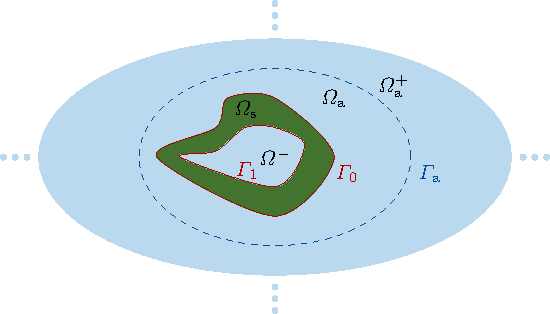
\includegraphics[scale=1]{artificialBoundary}
	\caption[Illustration of artificial boundary]{An artificial boundary $\Gamma_{\mathrm{a}}$ is introduced such that the exterior domain $\Omega^+$ is decomposed by the two domains $\Omega_{\mathrm{a}}$ (which is bounded by $\Gamma$ and $\Gamma_{\mathrm{a}}$) and $\Omega_{\mathrm{a}}^+$. Thus, $\Omega^+ = \Omega_{\mathrm{a}} \cup \Omega_{\mathrm{a}}^+$.}
	\label{Fig5:artificialBoundary}
\end{figure}
The exterior Helmholtz problem is given by
\begin{alignat}{3}
	\nabla^2 p + k^2 p &= 0 	&&\text{in}\quad \Omega^+,\label{Eq5:HelmholtzEqn}\\
	\partial_n p &= g						&&\text{on}\quad \Gamma,\label{Eq5:HelmholtzEqnNeumannCond}\\
	\pderiv{p}{r}-\imag k p &= o\left(r^{-1}\right)\quad &&\text{with}\quad r=|\vec{x}|\label{Eq5:sommerfeldCond}
\end{alignat}
where the Sommerfeld condition~\cite{Sommerfeld1949pde} in \Cref{Eq5:sommerfeldCond} restricts the field in the limit $r\to\infty$ uniformly in $\hat{\vec{x}}=\frac{\vec{x}}{r}$, such that no waves originate from infinity. The Neumann condition given by the function $g$ will in the case of rigid scattering be given by the incident wave $p_{\mathrm{inc}}$. Zero displacement of the fluid normal on the scatterer (rigid scattering) implies that $\partial_n(p+p_{\mathrm{inc}}) = 0$ where $\partial_n$ denotes the partial derivative in the normal direction on the surface $\Gamma$ (pointing ``out'' from $\Omega^+$), which implies that
\begin{equation}
	g = -\pderiv{p_{\mathrm{inc}}}{n}.
\end{equation}
Plane incident waves (with amplitude $\legendre_{\mathrm{inc}}$) traveling in the direction $\vec{d}_{\mathrm{s}}$ can be written as
\begin{equation}\label{Eq5:p_inc}
	p_{\mathrm{inc}}(\vec{x}) = \legendre_{\mathrm{inc}}\euler^{\imag k\vec{d}_{\mathrm{s}}\cdot\vec{x}}.
\end{equation}
The normal derivative on the surface of any smooth geometry may then be computed by
\begin{align}
	\pderiv{p_{\mathrm{inc}}}{n} &= \vec{n}\cdot\nabla p_{\mathrm{inc}} = \imag k\vec{d}_{\mathrm{s}}\cdot\vec{n} p_{\mathrm{inc}}.
\end{align}

The weak formulation for the Helmholtz problem can be shown to be (for details regarding the involved spaces, cf. \cite{Venas2018iao} and references therein)
\begin{equation}
	\text{Find} \quad p\in H_w^{1+}(\Omega^+)\quad\text{such that}\quad B(q,p) = L(q),\qquad \forall q\in H_{w^*}^1(\Omega^+),
\end{equation}
where the bilinear form is given by
\begin{equation}\label{Eq5:bilinear}
	B(q,p) = \int_{\Omega^+} \left[\nabla q\cdot\nabla p-  k^2qp\right]\idiff\Omega
\end{equation}
and the corresponding linear form is given by
\begin{equation*}
	L(q) = \int_{\Gamma} qg\idiff\Gamma.
\end{equation*}

The numerical solution (trial function) is expressed by the same Lagrange basis functions used to approximate the geometry
\begin{equation*}
	\hat{p}(\xi,\eta,\zeta) = \sum_{i=1}^{n_\upxi}\sum_{j=1}^{n_\upeta}\sum_{l=1}^{n_\upzeta}\hat{p}_{i,j,l} l_i(\xi)l_j(\eta)l_l(\zeta).
\end{equation*}
The parametric solution is related to the solution in the physical space by
\begin{equation*}
	\hat{p}(\xi,\eta,\zeta) = (p\circ \vec{C})(\xi,\eta,\zeta).
\end{equation*}
The derivatives are then given by the chain rule
\begin{equation*}
	\pderiv{\hat{p}}{\xi} = \pderiv{p}{x_1}\pderiv{F_1}{\xi} + \pderiv{p}{x_2}\pderiv{F_2}{\xi} + \pderiv{p}{x_3}\pderiv{F_3}{\xi} = \nabla p\cdot \pderiv{\vec{C}}{\xi}
\end{equation*}
and correspondingly for the other parametric derivatives such that
\begin{equation*}
	\hat{\nabla}\hat{p} = \vec{J}^\transpose\nabla p
\end{equation*}
where
\begin{equation*}
	\vec{J} = \begin{bmatrix}
		\pderiv{\vec{C}}{\xi} & \pderiv{\vec{C}}{\eta} & \pderiv{\vec{C}}{\zeta}
	\end{bmatrix} = \begin{bmatrix}
		\pderiv{C_1}{\xi} & \pderiv{C_1}{\eta} & \pderiv{C_1}{\zeta}\\
		\pderiv{C_2}{\xi} & \pderiv{C_2}{\eta} & \pderiv{C_2}{\zeta}\\
		\pderiv{C_3}{\xi} & \pderiv{C_3}{\eta} & \pderiv{C_3}{\zeta}
	\end{bmatrix}.
\end{equation*}
We therefore have
\begin{equation*}
	\nabla p = \vec{J}^{-\transpose}\hat{\nabla}\hat{p}.
\end{equation*}
Insertion of the trial function into the bilinear form (restricted to $\Omega_{\mathrm{a}}$) in \Cref{Eq5:bilinear} alongside test functions of the form
\begin{equation*}
	\hat{q}(\xi,\eta,\zeta) = l_{\tilde{i}}(\xi)l_{\tilde{j}}(\eta)l_{\tilde{l}}(\zeta),\quad 1\leq \tilde{i}\leq n_\upxi, \quad 1\leq \tilde{j}\leq n_\upeta, \quad 1\leq \tilde{l}\leq n_\upzeta
\end{equation*}
yields
\begin{equation*}\resizebox{\textwidth}{!}{$
\begin{aligned}
	B(q,p) &= \int_{\Omega_{\mathrm{a}}} \left(\nabla q\cdot\nabla p -  k^2qp\right)\idiff\Omega = \int_{-1}^1\int_{-1}^1\int_{-1}^1 \left((\hat{\nabla}\hat{q})^\transpose \vec{J}^{-1}\vec{J}^{-\transpose}\hat{\nabla}\hat{p} -  k^2\hat{q}\hat{p}\right)J\idiff\xi\idiff\eta\idiff\zeta\\
	&=  \sum_{i,j,l}\int_{-1}^1\int_{-1}^1\int_{-1}^1 \hat{p}_{i,j,l}\left([l'_{\tilde{i}}(\xi)l_{\tilde{j}}(\eta)l_{\tilde{l}}(\zeta), l_{\tilde{i}}(\xi)l'_{\tilde{j}}(\eta)l_{\tilde{l}}(\zeta), l_{\tilde{i}}(\xi)l_{\tilde{j}}(\eta)l'_{\tilde{l}}(\zeta)]\right.\\
	&{\hskip12em\relax}\left.\tilde{\vec{G}}[l'_i(\xi)l_j(\eta)l_l(\zeta), l_i(\xi)l'_j(\eta)l_l(\zeta), l_i(\xi)l_j(\eta)l'_l(\zeta)]^\transpose\right.\\
	&{\hskip11em\relax}\left. -  k^2l_{\tilde{i}}(\xi)l_{\tilde{j}}(\eta)l_{\tilde{l}}(\zeta)l_i(\xi)l_j(\eta)l_l(\zeta)J\right)\idiff\xi\idiff\eta\idiff\zeta\\
	&\approx \sum_{i,j,l}\hat{p}_{i,j,l}\sum_{\alpha\beta\gamma} \left([l'_{\tilde{i}}(\xi_\alpha)l_{\tilde{j}}(\eta_\beta)l_{\tilde{l}}(\zeta_\gamma), l_{\tilde{i}}(\xi_\alpha)l'_{\tilde{j}}(\eta_\beta)l_{\tilde{l}}(\zeta_\gamma), l_{\tilde{i}}(\xi_\alpha)l_{\tilde{j}}(\eta_\beta)l'_{\tilde{l}}(\zeta_\gamma)]\right.\\
	&{\hskip8em\relax}\left.\tilde{\vec{G}}_{\alpha\beta\gamma}[l'_i(\xi_\alpha)l_j(\eta_\beta)l_l(\zeta_\gamma), l_i(\xi_\alpha)l'_j(\eta_\beta)l_l(\zeta_\gamma), l_i(\xi_\alpha)l_j(\eta_\beta)l'_l(\zeta_\gamma)]^\transpose\right.\\
	&{\hskip7em\relax}\left. -  k^2l_{\tilde{i}}(\xi_\alpha)l_{\tilde{j}}(\eta_\beta)l_{\tilde{l}}(\zeta_\gamma)l_i(\xi_\alpha)l_j(\eta_\beta)l_l(\zeta_\gamma)J_{\alpha\beta\gamma}\right)\\
	&= \sum_{i,j,l}\hat{p}_{i,j,l}\sum_{\alpha\beta\gamma} \left([D_{\tilde{i}\alpha}^\Xi\delta_{\tilde{j}\beta}\delta_{\tilde{l}\gamma}, \delta_{\tilde{i}\alpha}D_{\tilde{j}\beta}^\Eta\delta_{\tilde{l}\gamma}, \delta_{\tilde{i}\alpha}\delta_{\tilde{j}\beta}D_{\tilde{l}\gamma}^\Zeta]\tilde{\vec{G}}_{\alpha\beta\gamma}[D_{i\alpha}^\Xi\delta_{j\beta}\delta_{l\gamma}, \delta_{i\alpha}D_{j\beta}^\Eta\delta_{l\gamma}, \delta_{i\alpha}\delta_{j\beta}D_{l\gamma}^\Zeta]^\transpose\right.\\
	&{\hskip7em\relax}\left. -  k^2\delta_{\tilde{i}\alpha}\delta_{\tilde{j}\beta}\delta_{\tilde{l}\gamma}\delta_{i\alpha}\delta_{j\beta}\delta_{l\gamma}J_{\tilde{i}\tilde{j}\tilde{l}}\right)\\
	&= -  k^2 \rho_{\tilde{i}}\rho_{\tilde{j}}\rho_{\tilde{l}}\hat{p}_{\tilde{i},\tilde{j},\tilde{l}}J_{\tilde{i}\tilde{j}\tilde{l}} + \sum_{i,j,l}\hat{p}_{i,j,l}\sum_{\alpha\beta\gamma} w_{ijl\alpha\beta\gamma\tilde{i}\tilde{j}\tilde{l}}
\end{aligned}	
	$}
\end{equation*}
where
\begin{equation*}\resizebox{\textwidth}{!}{$
\begin{aligned}
	&J_{\alpha\beta\gamma} = J(\xi_\alpha,\eta_\beta,\zeta_\gamma),\quad J = \det{\vec{J}}, \quad\tilde{\vec{G}}_{\alpha\beta\gamma} = \rho_\alpha\rho_\beta\rho_\gamma\tilde{\vec{G}}(\xi_\alpha,\eta_\beta,\zeta_\gamma),\\
	&\tilde{\vec{G}} = J\vec{G},\quad\vec{G} = \vec{J}^{-1}\vec{J}^{-\transpose}\quad D_{i\alpha}^\Xi = l'_{i}(\xi_\alpha),\quad D_{j\beta}^\Eta = l'_{j}(\eta_\beta),\quad D_{l\gamma}^\Zeta = l'_l(\zeta_\gamma)\\
	&w_{ijl\alpha\beta\gamma\tilde{i}\tilde{j}\tilde{l}} = [D_{\tilde{i}\alpha}^\Xi\delta_{\tilde{j}\beta}\delta_{\tilde{l}\gamma}, \delta_{\tilde{i}\alpha}D_{\tilde{j}\beta}^\Eta\delta_{\tilde{l}\gamma}, \delta_{\tilde{i}\alpha}\delta_{\tilde{j}\beta}D_{\tilde{l}\gamma}^\Zeta]\tilde{\vec{G}}_{\alpha\beta\gamma}[D_{i\alpha}^\Xi\delta_{j\beta}\delta_{l\gamma}, \delta_{i\alpha}D_{j\beta}^\Eta\delta_{l\gamma}, \delta_{i\alpha}\delta_{j\beta}D_{l\gamma}^\Zeta]^\transpose.
\end{aligned}	
	$}
\end{equation*}
For a set of indices $i,j,l,\tilde{i},\tilde{j},\tilde{l}$, we have
\begin{equation*}\resizebox{\textwidth}{!}{$
\begin{aligned}
	\sum_{\alpha\beta\gamma} w_{ijl\alpha\beta\gamma\tilde{i}\tilde{j}\tilde{l}} &= \sum_{\alpha\beta\gamma}  [D_{\tilde{i}\alpha}^\Xi\delta_{\tilde{j}\beta}\delta_{\tilde{l}\gamma}, \delta_{\tilde{i}\alpha}D_{\tilde{j}\beta}^\Eta\delta_{\tilde{l}\gamma}, \delta_{\tilde{i}\alpha}\delta_{\tilde{j}\beta}D_{\tilde{l}\gamma}^\Zeta]\tilde{\vec{G}}_{\alpha\beta\gamma}[D_{i\alpha}^\Xi\delta_{j\beta}\delta_{l\gamma}, \delta_{i\alpha}D_{j\beta}^\Eta\delta_{l\gamma}, \delta_{i\alpha}\delta_{j\beta}D_{l\gamma}^\Zeta]^\transpose\\
	&= \sum_{\alpha\beta\gamma}  \left(\left[(\tilde{G}_{11})_{\alpha\beta\gamma} D_{i\alpha}^\Xi\delta_{j\beta}\delta_{l\gamma} +(\tilde{G}_{12})_{\alpha\beta\gamma} \delta_{i\alpha}D_{j\beta}^\Eta\delta_{l\gamma} + (\tilde{G}_{13})_{\alpha\beta\gamma} \delta_{i\alpha}\delta_{j\beta}D_{l\gamma}^\Zeta\right]D_{\tilde{i}\alpha}^\Xi\delta_{\tilde{j}\beta}\delta_{\tilde{l}\gamma}\right.\\	
	&{\hskip3em\relax}+\left[(\tilde{G}_{21})_{\alpha\beta\gamma} D_{i\alpha}^\Xi\delta_{j\beta}\delta_{l\gamma} + (\tilde{G}_{22})_{\alpha\beta\gamma} \delta_{i\alpha}D_{j\beta}^\Eta\delta_{l\gamma} + (\tilde{G}_{23})_{\alpha\beta\gamma} \delta_{i\alpha}\delta_{j\beta}D_{l\gamma}^\Zeta\right] \delta_{\tilde{i}\alpha}D_{\tilde{j}\beta}^\Eta\delta_{\tilde{l}\gamma}\\	
	&{\hskip3em\relax}+\left.\left[(\tilde{G}_{31})_{\alpha\beta\gamma} D_{i\alpha}^\Xi\delta_{j\beta}\delta_{l\gamma} +(\tilde{G}_{32})_{\alpha\beta\gamma} \delta_{i\alpha}D_{j\beta}^\Eta\delta_{l\gamma} + (\tilde{G}_{33})_{\alpha\beta\gamma} \delta_{i\alpha}\delta_{j\beta}D_{l\gamma}^\Zeta\right] \delta_{\tilde{i}\alpha}\delta_{\tilde{j}\beta}D_{\tilde{l}\gamma}^\Zeta\right)\\
	&= \delta_{\tilde{l}l} (\tilde{G}_{12})_{i\tilde{j}l} D_{\tilde{i}i}^\Xi  D_{j\tilde{j}}^\Eta
	+ \delta_{\tilde{j}j} (\tilde{G}_{13})_{ij\tilde{l}} D_{\tilde{i}i}^\Xi D_{l\tilde{l}}^\Zeta
	+ \delta_{\tilde{j}j}\delta_{\tilde{l}l}\sum_{\alpha=1}^{n_\upxi} (\tilde{G}_{11})_{\alpha jl} D_{i\alpha}^\Xi D_{\tilde{i}\alpha}^\Xi \\
	&\quad+ \delta_{\tilde{l}l} (\tilde{G}_{12})_{\tilde{i} jl}D_{i\tilde{i}}^\Xi D_{\tilde{j}j}^\Eta
	+ \delta_{\tilde{i}i}  (\tilde{G}_{23})_{ij\tilde{l}}  D_{\tilde{j}j}^\Eta D_{l\tilde{l}}^\Zeta
	+ \delta_{\tilde{i}i}\delta_{\tilde{l}l}\sum_{\beta=1}^{n_\upeta}(\tilde{G}_{22})_{i\beta l} D_{j\beta}^\Eta D_{\tilde{j}\beta}^\Eta\\
	&\quad+ \delta_{\tilde{j}j} (\tilde{G}_{13})_{\tilde{i}jl}D_{i\tilde{i}}^\Xi D_{\tilde{l}l}^\Zeta
	+ \delta_{\tilde{i}i} (\tilde{G}_{23})_{i\tilde{j} l}D_{j\tilde{j}}^\Eta D_{\tilde{l}l}^\Zeta
	+ \delta_{\tilde{i}i}\delta_{\tilde{j}j}\sum_{\gamma=1}^{n_\upzeta} (\tilde{G}_{33})_{ij\gamma}D_{l\gamma}^\Zeta D_{\tilde{l}\gamma}^\Zeta
\end{aligned}	
	$}
\end{equation*}
where we have exploited the symmetry of $\tilde{\vec{G}}$. Although the 1D stiffness matrix for an element is fully dense, this is not the case for higher dimensional SEM stiffness matrices. This is again due to \Cref{Eq5:LagrangeProperty}. An upper bound on the number of non-zero elements in the stiffness matrix can be shown to be $n_\upxi n_\upeta^2 n_\upzeta^2+n_\upxi^2 n_\upeta n_\upzeta^2+n_\upxi n_\upeta^2 n_\upzeta$. Defining $n=\max\{n_\upxi, n_\upeta, n_\upzeta\}$, then an lower bound on the sparsity of the stiffness matrix is $1-d/n$ (with $d$ being the dimension of the problem), meaning the sparsity is increased as a function of the number of degrees of freedom. This is in stark contrast to an IGA element matrix which will in general be fully dense (cf.  \cite{Gervasio2018cia}) when pure $\check{p}$-refinement is used.

For the linear form, we simply get (assuming the boundary $\Gamma$ is parameterized by $\xi$ and $\eta$ at $\zeta = 0$)
\begin{equation*}
	L(q) = \int_{\Gamma} qg\idiff\Gamma =  \rho_{\tilde{i}}\rho_{\tilde{j}}\hat{g}_{\tilde{i}\tilde{j}}H_{\tilde{i}\tilde{j}}\delta_{0\tilde{l}}.
\end{equation*}
where
\begin{equation*}
	\hat{g}_{\alpha,\beta} = (g\circ \vec{C})(\xi_\alpha,\eta_\beta,-1),\quad H_{\alpha\beta} = H(\xi_\alpha,\eta_\beta), \quad H(\xi,\eta) = \left\|\pderiv{\vec{C}|_\Gamma}{\xi}\times\pderiv{\vec{C}|_\Gamma}{\eta}\right\|.
\end{equation*}
In order to evaluate the derivatives of the mapping $\vec{C}$ at the GLL nodes we note that
\begin{equation*}
	\left.\pderiv{\vec{C}}{\xi}\right|_{(\xi_\alpha,\eta_\beta,\zeta_\gamma)} = \sum_{i,j,l}\vec{c}_{i,j,l} l'_i(\xi_\alpha)l_j(\eta_\beta)l_l(\zeta_\gamma) = \sum_{i=1}^{n_\upxi}\vec{c}_{i,\beta,\gamma} l'_i(\xi_\alpha).
\end{equation*}
If we then store the derivatives $l'_i(\xi_\alpha)$ in the matrix $\vec{D}^\Xi\in\R^{n_\upxi\times n_\upxi}$ all evaluations may be done efficiently by the matrix-matrix products $\vec{D}^\Xi\vec{c}$ where the multidimensional array $\vec{c}\in\R^{3\times n_\upxi\times n_\upeta\times n_\upzeta}$ is the collection of all coefficients of $\vec{C}$. Note that $\vec{c}$ must be rearranged in order to make sense of the product with $\vec{D}^\Xi$. Corresponding efficient evaluations of the other derivatives at the GLL points can be performed in a similar procedure. 

The contributions from the infinite elements can be correspondingly efficiently evaluated using the following formulas
\begin{equation*}\resizebox{\textwidth}{!}{$
\begin{aligned}
	A_{ij\tilde{i}\tilde{j}}^{(1)} &= \int_{-1}^1\int_{-1}^1 l_i(\xi)l_j(\eta)l_{\tilde{i}}(\xi)l_{\tilde{j}}(\eta)\sin[\vartheta(\xi,\eta)]J^{(3)}(\xi,\eta)\idiff\xi\idiff\eta \\
	&\approx \delta_{i\tilde{i}}\delta_{j\tilde{j}}\rho_{\tilde{i}}\rho_{\tilde{j}}\sin\vartheta_{\tilde{i}\tilde{j}}J_{\tilde{i}\tilde{j}}^{(3)}\\
	A_{ij\tilde{i}\tilde{j}}^{(2)} &= \int_{-1}^1\int_{-1}^1 \left[J_{11}^{(5)}l_i'l_{\tilde{i}}'l_j l_{\tilde{j}} + J_{12}^{(5)}\left(l_i'l_{\tilde{i}}l_jl_{\tilde{j}}' + l_il_{\tilde{i}}'l_j'l_{\tilde{j}}\right) + J_{13}^{(5)}l_i l_{\tilde{i}}l_j'l_{\tilde{j}}'\right]\sin\vartheta\idiff\xi\idiff\eta\\
	&\approx \delta_{j\tilde{j}}\sum_{\alpha=1}^{n_\upxi} J_{11,\alpha j}^{(5)}D_{i\alpha}^\Xi D_{\tilde{i}\alpha}^\Xi + J_{12,\tilde{i}j}^{(5)}D_{i\tilde{i}}^\Xi D_{\tilde{j}j}^\Eta + J_{12,i\tilde{j}}^{(5)}D_{\tilde{i}i}^\Xi D_{j\tilde{j}}^\Eta + \delta_{i\tilde{i}}\sum_{\beta=1}^{n_\upeta} J_{13,i\beta}^{(5)}D_{j\beta}^\Eta D_{\tilde{j}\beta}^\Eta \\
	A_{ij\tilde{i}\tilde{j}}^{(3)} &= \int_{-1}^1\int_{-1}^1 l_i(\xi)l_j(\eta)l_{\tilde{i}}(\xi)l_{\tilde{j}}(\eta)\sin[\vartheta(\xi,\eta)]J_3(\xi,\eta)\idiff\xi\idiff\eta\\
	&\approx \delta_{i\tilde{i}}\delta_{j\tilde{j}}\rho_{\tilde{i}}\rho_{\tilde{j}}\cos^2\vartheta_{\tilde{i}\tilde{j}}\sin\vartheta_{\tilde{i}\tilde{j}}J_{\tilde{i}\tilde{j}}^{(3)}\\
	A_{ij\tilde{i}\tilde{j}}^{(4)} &= \int_{-1}^1\int_{-1}^1 \left[J_{21}^{(5)}l_i'l_{\tilde{i}}'l_j l_{\tilde{j}} + J_{22}^{(5)}\left(l_i'l_{\tilde{i}}l_jl_{\tilde{j}}' + l_il_{\tilde{i}}'l_j'l_{\tilde{j}}\right) + J_{23}^{(5)}l_i l_{\tilde{i}}l_j'l_{\tilde{j}}'\right]\frac{1}{\sin\vartheta}\idiff\xi\idiff\eta\\
	&\approx \delta_{j\tilde{j}}\sum_{\alpha=1}^{n_\upxi} J_{21,\alpha j}^{(5)}D_{i\alpha}^\Xi D_{\tilde{i}\alpha}^\Xi + J_{22,\tilde{i}j}^{(5)}D_{i\tilde{i}}^\Xi D_{\tilde{j}j}^\Eta + J_{22,i\tilde{j}}^{(5)}D_{\tilde{i}i}^\Xi D_{j\tilde{j}}^\Eta + \delta_{i\tilde{i}}\sum_{\beta=1}^{n_\upeta} J_{23,i\beta}^{(5)}D_{j\beta}^\Eta D_{\tilde{j}\beta}^\Eta \\
	A_{ij\tilde{i}\tilde{j}}^{(5)} &= \int_{-1}^1\int_{-1}^1 \left[J_{21}^{(5)}l_i'l_{\tilde{i}}'l_j l_{\tilde{j}} + J_{22}^{(5)}\left(l_i'l_{\tilde{i}}l_jl_{\tilde{j}}' + l_il_{\tilde{i}}'l_j'l_{\tilde{j}}\right) + J_{23}^{(5)}l_i l_{\tilde{i}}l_j'l_{\tilde{j}}'\right]\frac{\cos^2\theta}{\sin\vartheta}\idiff\xi\idiff\eta\\
	&\approx \delta_{j\tilde{j}}\sum_{\alpha=1}^{n_\upxi} J_{31,\alpha j}^{(5)}D_{i\alpha}^\Xi D_{\tilde{i}\alpha}^\Xi + J_{32,\tilde{i}j}^{(5)}D_{i\tilde{i}}^\Xi D_{\tilde{j}j}^\Eta + J_{32,i\tilde{j}}^{(5)}D_{\tilde{i}i}^\Xi D_{j\tilde{j}}^\Eta + \delta_{i\tilde{i}}\sum_{\beta=1}^{n_\upeta} J_{33,i\beta}^{(5)}D_{j\beta}^\Eta D_{\tilde{j}\beta}^\Eta
\end{aligned}	
	$}
\end{equation*}
where
\begin{align*}
	 J^{(5)}_{1j,\alpha\beta} &= \rho_\alpha\rho_\beta\sin\theta_{\alpha\beta} J^{(5)}_{1j}(\xi_\alpha,\eta_\beta),\quad J^{(5)}_{2j,\alpha\beta} = \frac{\rho_\alpha\rho_\beta}{\sin\theta_{\alpha\beta} } J^{(5)}_{2j}(\xi_\alpha,\eta_\beta),\\
	 J^{(5)}_{3j,\alpha\beta} &= \rho_\alpha\rho_\beta\frac{\cos^2\theta_{\alpha\beta}}{\sin\theta_{\alpha\beta} } J^{(5)}_{2j}(\xi_\alpha,\eta_\beta),\quad
	 \vec{J}^{(4)} = \begin{bmatrix}
	 	J_{11}^{(4)} & J_{12}^{(4)}\\
	 	J_{21}^{(4)} & J_{22}^{(4)}
\end{bmatrix}	\defeq  \left[\vec{J}^{(3)}\right]^{-\transpose}\\
	 \vec{J}^{(5)} &= \begin{bmatrix}
	 	J_{11}^{(5)} & J_{12}^{(5)} & J_{13}^{(5)}\\
	 	J_{21}^{(5)} & J_{22}^{(5)} & J_{23}^{(5)}
\end{bmatrix} \defeq J^{(3)}\begin{bmatrix}
	 	J_{11}^{(4)}J_{11}^{(4)} & J_{12}^{(4)}J_{11}^{(4)} & J_{12}^{(4)}J_{12}^{(4)}\\
	 	J_{21}^{(4)}J_{21}^{(4)} & J_{22}^{(4)}J_{21}^{(4)} & J_{22}^{(4)}J_{22}^{(4)}
	 \end{bmatrix}
\end{align*}
where $\theta_{\alpha\beta}$ is the polar angle (evaluated using~\cite[Equation (A.4)]{Venas2018iao}) at the GLL point $\vec{X}(\xi_\alpha,\eta_\beta,1)$. 